\documentclass[12pt,a4paper]{article}

\usepackage[utf8]{inputenc}
\usepackage{graphicx}
\usepackage[spanish]{babel}
\usepackage{float}				%Para poner las imagenes exactamente donde se me cante las pelotas en caso de quererlo, poniendole [H]
\usepackage{amsmath}
\usepackage{epstopdf}
\usepackage{geometry}
\usepackage{hieroglf}
\usepackage{subcaption}
\usepackage[justification=centering]{caption}
\usepackage[colorlinks=true, allcolors=blue]{hyperref}
\geometry{
a4paper,
left=20mm,
right=20mm,
top=25mm,
bottom = 20mm
}
\usepackage{float}
\usepackage{units}
\marginparwidth=2cm
\usepackage[colorinlistoftodos]{todonotes}

% \usepackage{hyperref}   %Esto es para ir a los links

\title{\mathbf{Elementos Finitos \\Práctica 2}}
\author{Universidad de Cuenca}
\begin{document}
\maketitle
\begin{enumerate}
    \item Emplear el código implementado en la práctica anterior para resolver el problema de una varilla de área variable como la de la figura, cuyo módulo de Young es $E=2x10^7Pa$ y se encuentra sometida a una fuerza de estiramiento $b=10Nm^{-1}$ entre los puntos  A y B y una fuerza puntual $P=150N$ en el punto C. El área entre los puntos A y B es igual a $0.1 m^2$ y entre B y C sigue la ecuación $A(x)=(0.5x-1)m^2$. Las medidas de x en la figura están en metros. Resolver con 2,4 y 10 elementos. Comparar los resultados.
    \begin{figure}[H]
        \centering
        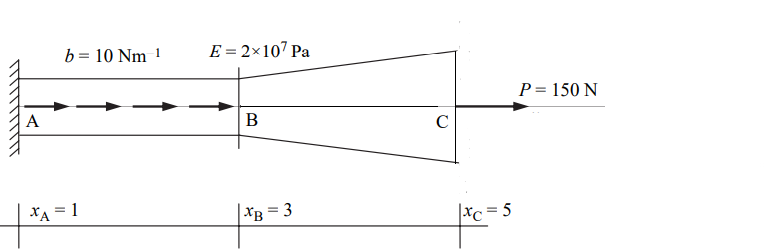
\includegraphics[width=0.8\textwidth]{tp2-1.png}
        \label{fig:ejercicio1}
    \end{figure}
\end{enumerate}

\end{document}